\section{Results}
\label{sec:results}
\begin{table*}[t]
\centering\small
\begin{tabular}{lrrrrrr}
\toprule
Method & EM (\%) & F1 (\%) & Utility & Tokens / $S$ item & Pairs & Correct / break \\
\midrule
Closure EVSI (nominee) & 60.508 & 71.295 & 0.567215 & 7572.58 & 6.350 & 70 / 73 \\
EVSI fixed price & 60.508 & 71.295 & 0.567048 & 7606.07 & 6.300 & 70 / 73 \\
EVSI no cost ranking & 60.508 & 71.295 & 0.567041 & 7607.40 & 6.350 & 70 / 73 \\
EVSI old graph cost & 60.898 & 71.592 & 0.569451 & 7906.63 & 6.300 & 73 / 66 \\
Random & 60.508 & 71.266 & 0.566282 & 7759.20 & 8.000 & 71 / 74 \\
Periodic & 60.352 & 71.100 & 0.566172 & 7468.82 & 8.000 & 71 / 78 \\
Uncertainty & 60.547 & 71.315 & 0.566661 & 7761.61 & 8.000 & 70 / 72 \\
Changed first & 60.781 & 71.418 & 0.567563 & 8049.98 & 8.000 & 75 / 71 \\
Stale & 60.508 & 71.184 & 0.571291 & 6757.50 & 0.000 & 74 / 77 \\
Protect changed & 61.641 & 72.579 & 0.576462 & 7988.82 & 0.000 & 73 / 47 \\
Keep (with init.) & 60.625 & 71.245 & 0.565966 & 8056.70 & 0.000 & 0 / 0 \\
Keep (no init.) & 60.625 & 71.245 & 0.572537 & 6742.51 & 0.000 & 0 / 0 \\
Delete changed (no init.) & 60.117 & 70.617 & 0.575727 & 5088.94 & 0.000 & 71 / 84 \\
Delete other (no init.) & 61.797 & 72.744 & 0.584613 & 6671.07 & 0.000 & 78 / 48 \\
Single Qwen & 57.578 & 65.539 & 0.568207 & 1514.93 & 0.000 & 267 / 345 \\
Vote Qwen (3) & 57.891 & 65.895 & 0.556182 & 4544.88 & 0.000 & 272 / 342 \\
Independent 3 + Qwen & 58.984 & 70.520 & 0.556352 & 6698.34 & 0.000 & 178 / 220 \\
\bottomrule
\end{tabular}
\caption{Graph-change service results. Each method has 512 distinct service questions and 2,560 question--seed observations. Tokens include initialization and feedback; pairs are per episode--seed. Corrections/breakages use the matched keep output. No uncertainty intervals are shown.}
\label{tab:change}
\end{table*}

\begin{table}[t]
\centering\small
\begin{tabular}{lrrr}
\toprule
Seed & EM (\%) & $J$ & $J-J_{\rm random}$ \\
\midrule
26111571 & 61.133 & 0.572538 & +0.005428 \\
26111572 & 58.984 & 0.552394 & +0.001216 \\
26111573 & 61.719 & 0.579941 & -0.000022 \\
26111574 & 60.938 & 0.570770 & -0.002798 \\
26111575 & 59.766 & 0.560433 & +0.000841 \\
\bottomrule
\end{tabular}
\caption{All five nominee seeds under graph change. Seeds share the same question groups.}
\label{tab:seeds}
\end{table}

\paragraph{Complete execution and verification.}
All 640 questions completed with 28,800 terminal answers, 99,200 logical
node calls, and 47,640 physical generations after exact request reuse.
All terminal answers were nonempty and ended at an end-of-sequence token.
The archived collection contains 1,942 hash-verified files. Request replay
matched 913,924 fields; separate implementations passed 626,080
policy/cost/point checks and 89,692 raw scoring/voting checks. These checks
use recorded generations and do not constitute new stochastic replications.
Formal collection consumed 25.210263 GPU residence hours, with a separately
charged 0.066123-hour qualification.

\paragraph{The nominee fails the frozen admission rule.}
Table~\ref{tab:change} reports every strategy under graph change.
Closure EVSI and random revalidation both achieve 60.5078125\% exact match.
The utility difference is only $+0.000933084$, below the required $+0.005$.
It is positive for three of five seeds, below the required four
(Table~\ref{tab:seeds}). The nominee is worse in utility than stale credit
by 0.004075416, protect-changed by 0.009246910, and no-initialization keep
by 0.005322254. Thus acquiring feedback has not established incremental
value beyond inexpensive decisions in this setting.

Relative to single Qwen, the nominee gains 2.929688 percentage points (pp)
in exact match but uses 4.998639 times the complete tokens, yielding a
utility difference of $-0.000991387$. Relative to independent-three
aggregation, it gains 1.523438 pp, but its token ratio is 1.130516 rather
than the required at most 0.90. The independent-aggregation quality and
voting-utility gates pass; the other four gates fail. We retain the frozen
stop decision and do not promote a better-looking control.

\paragraph{Ablations do not establish the proposed mechanism's value.}
Fixed-price EVSI and EVSI without cost-normalized ranking have exactly
the same aggregate exact match as the nominee. The nominee's utility
advantages are $+0.000167461$ and $+0.000174094$, respectively. Using
old-graph service prices produces higher exact match and higher utility
than the nominee here; the nominee's utility difference is
$-0.002236002$. These are descriptive comparisons, not evidence that
the old-price ablation is a newly validated method.

The nominee corrects 70 keep errors but breaks 73 keep successes across
2,560 paired question--seed observations. Its net correctness change from
keep is therefore $-3/2560$. These output-level counterfactual counts do
not identify the true expected sign of each edge's credit.

\paragraph{No-change and cost controls.}
Without the exogenous shock, the nominee reaches 60.429688\% exact match
and utility 0.560880619 (Appendix Table~\ref{tab:no_change}). Its utility is
0.003030441 below stale credit. The observed result therefore does not
support a robust advantage outside the shock condition either.
No-initialization deletion of the other direct edge is the strongest
point estimate in Table~\ref{tab:change}, but it is an already specified
control, not a replacement winner or independently confirmed policy.

The nominee pays 3,364,346 initialization tokens, 1,473,212 feedback tokens,
and 14,548,249 service tokens across its 40 graph-change episode--seed runs.
The total is 19,385,807 tokens, or 7,572.58 per service observation.
Its mean feedback count is 6.35 pairs, compared with eight for random.
Figure~\ref{fig:cost} displays all seed points and utility differences.
Appendix Table~\ref{tab:weights} reports the predeclared weight sensitivity
without changing the primary weight or selecting a new policy.

\begin{figure*}[t]
\centering
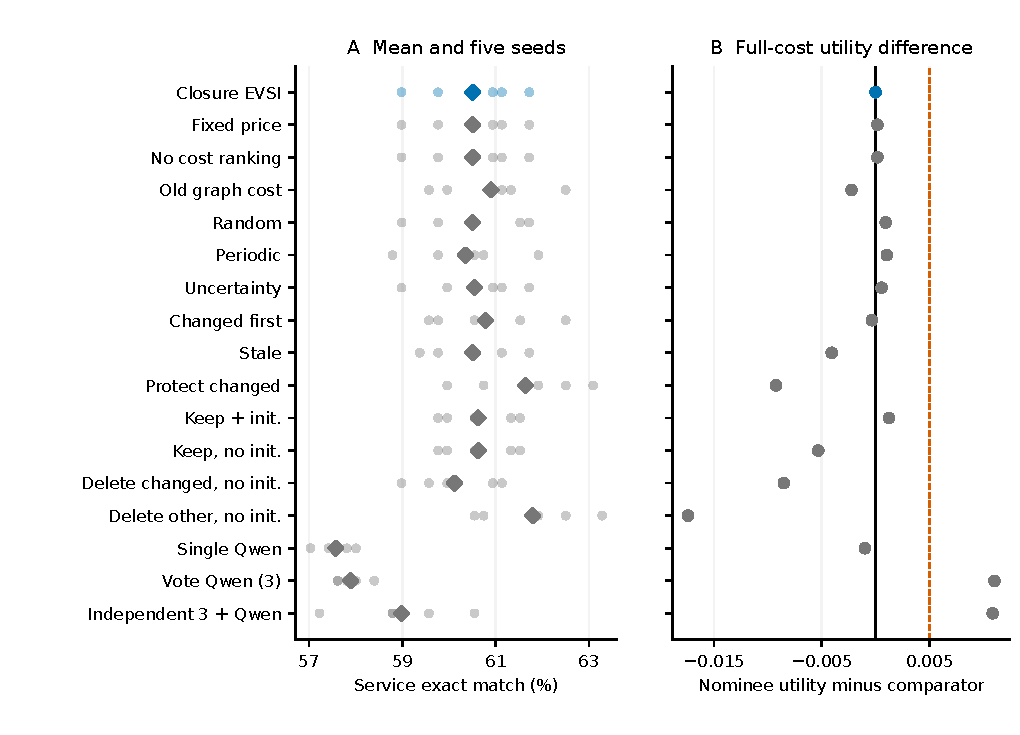
\includegraphics[width=\textwidth]{figures/paper_points.pdf}
\caption{Graph-change point estimates and nominee-minus-comparator utility. Diamonds show mean exact match; small points show all five seeds. The dashed line marks the required $+0.005$ gain for the designated maintenance/free controls; other system gates differ. Complete utility charges initialization, feedback, and service. There are no confidence intervals.}
\label{fig:cost}
\end{figure*}
